\chapter{Implementation and Testing}
Following the formal definition of the Lispish language and briefly describing the operations of the compiler, we shall dive into the construction of it. Along the way, I will explain the concepts behind most of the mechanics of the compiler. 

In the following sections, we will also test the implementation by means of examples of an actual compilation. 
At the end, we will look into automating the tests by means of using a Clojure testing API.  

\section{Building the compiler}
This section will describe the operations of the compiler and the fundamental concepts behind how the compiler translates the input Lispish code to JavaScript. 

Lispish translator is implemented as a single pass compiler.
This design decision comes from the fact that the compiler has been implemeneted in Clojure, which is a strictly functional language and in order to sustain the immutability property throughout the compiler and not violate common idioms, the compiler avoids using state at all costs. It was therefore difficult to perform multi-pass compilation over the same code, as it is done in other commercial compilers. 
As a consequence of this, the entire implementation is built around recursively invoking a set a functions, which at the end fold to yield a JavaScript string as a result. 

\subsection{Abstract Structural Binding}
Abstract Structural Binding allows for de-structuring any data structure to a corresponding argument in function parameters or a let form, creating locally scoped bindings.
For example, if we define a let as follows:
\begin{verbatim}
(let [[x1 x2] [1 2]])
\end{verbatim}
\texttt{x1} will yield \texttt{1} and \texttt{x2} will yield \texttt{2}.
The same principle is true for a function.
If our function accepts one parameter which is a collection:

\begin{verbatim}
(defn test [[x1 x2]] (println x1 x2))
(test [1])
\end{verbatim}
and it binds the first two elements of the collection to x1 x2, in the above case, x1 will yield 1 and x2 null.

Lispish uses de-structuring for generating all of its forms. 
Take for instance the signature of a \texttt{(emit-defn)} function responsible for expanding and generating the equivalent JavaScript named function code:
$$ \texttt{(defn emit-defn [type [defn name [arg \& more] \& rest]] )} $$

In order to split the provided input source code \texttt{(defn ))} form into its respective elements, the  performs a structural binding of the function arguments. The bindings are then used to generate the equivalent JavaScript code. 

as we can see, the function takes 4 arguments and 2 optional tail arguments that can be a list of an arbitrary length. The \texttt{type} argument is simply a convenience placeholder for the head of the whole expression.
The actual expression begins to bind from the [defn name [arg \& more] \& rest] arguments. 

\begin{figure}[ht]
\centering
\begin{verbatim}
(defn emit-defn [type [defn name [arg & more] & rest]]
    (str "function " (if (= "~" name) "" name) "("
     
         ;; Output the argument names 
         (if (nil? more) arg (str arg ", " (clojure.string/join ", " more)))
          ") {return "
        
         ;; Emit body of the function
         (emit rest)

         "}")))
\end{verbatim}
\caption{Emit-defn function}
\label{fig:emit-defn}
\end{figure}


Figure ~\ref{fig:emit-defn} illustrates the body of the \texttt{(emit-defn)} function and how the bindings acquired upon the function call are used to then generate the corresponding JavaScript quite. 
At first, we are checking if the \texttt{name} binding is a \texttt{~} character, which is a special case meaning that the function is anonymous (we are passing it from the emit-fn with the rest of the expression, to decrease code count) and an empty string in place of the function name needs to be generated. The function then outputs the argument names. In case if there are multiple arguments, it will output an arguments string with the arguments separated by commas. 
At the end it emits the body \texttt{(emit rest)} of the function.

The optional \texttt{more} in the arguments list allows for an arbitrary length of the function arguments and the optional rest is for the expression that follows the named function.

\subsection{Recursive Expansion}
The main idea behind the Lispish compiler's implementation is recursive expansion.
The compiler breaks down each s-expression that it comes across into its primitives until there is no more work to be done. It then builds up the result in layers as the recursion folds upwards. 

Figure ~\ref{fig:recursive_expansion_flowchart} illustrates the flow chart of the compiler. It covers most of the operations of the compiler, except for the details on how multi-arity s-expressions are handled.  

\begin{figure}[!htbp]
	\centering
	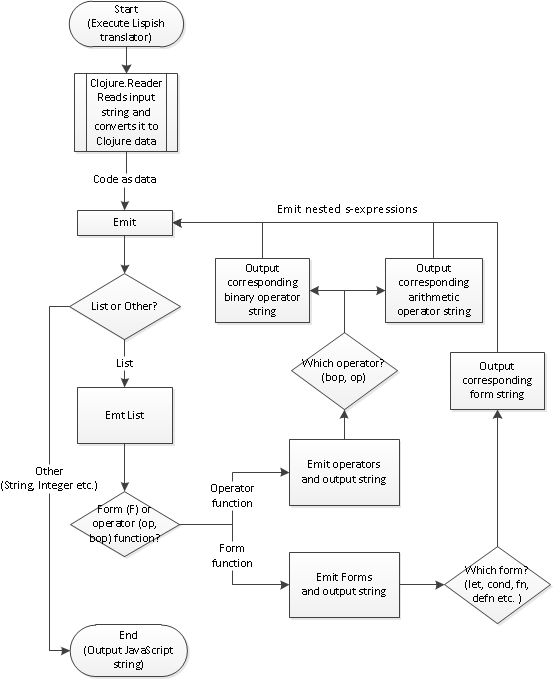
\includegraphics{Graphics/compilation_flow_chart.png}
	\caption[yadayada]
   {Flow chart of \textit{Lispish to JavaScript} compilation.}
  \label{fig:recursive_expansion_flowchart}
\end{figure}

To illustrate how in practice the recursive expansion is performed, lets consider how a single form gets expanded and also how its equivalent JavaScript code is generated. 

\begin{figure}[ht]
\begin{verbatim}
(defn emit [expressions]
  "Take an s-expression and emit its corresponding JavaScript form"
  (do
    (println "Emit Lispish: " expressions)
    (cond
      (nil? expressions) "null"
      (symbol? expressions) (str expressions)
      (seq? expressions) (emit-list expressions)
      (integer? expressions) (str expressions)
      (float? expressions) (str expressions)
      (string? expressions) (str expressions)
      :else (str expressions))))
\end{verbatim}
\caption{Top level function of the recursive expansion}
\label{fig:emit}
\end{figure}

Figure ~\ref{fig:emit} is the top level function of the recursive translator. It is responsible for determining s-expression's type. This is possible as whenever the translator gets executed and a source file is provided as its input, the Clojure Reader is used to read the input source and as a result, it outputs the code as data, more precisely, as lists. 
These lists can be then checked for type, as the Clojure Reader is responsible for parsing and giving each symbol its corresponding type.

As illustrated on the ~\ref{fig:recursive_expansion_flowchart} flowchart, there is indeed two cases for the emit function. The argument is either a list and it therefore needs to be expanded or it's one of the generic types, e.g. Integer or String and therefore needs to be outputted as a string already at this point. 

\subsection{Forms with multiple arity}

In order to solve the multiple arity problem, where for instance a \texttt{(cond )} form can take multiple condition/true-form expression tuples and each one of them has to be compiler to a JavaScript string, map and reduce constructs have been used. 

\subsubsection{Map}
The idea behind the map operation is to apply a function that takes one argument, to all of the elements in a collection and return a new collection with results of each application of the aforementioned function. 
A simple example of Map is 

\begin{verbatim}
(map (fn [x] (+ x 1)) 
	 [0 1 2 3 4 5])
\end{verbatim}
that yields 
\begin{verbatim}
[1 2 3 4 5 6]
\end{verbatim}
as a result

\subsubsection{Reduce}
Reduce is a function that takes a function, an optional value (or an s-expression) and a collection as an argument. It reduces or in other words folds a given collection (and an optional value) through the application of a function to a collection, to a single result. 
\begin{verbatim}
(reduce 
   str
   1
	 [1 2 3])
\end{verbatim}
that yields 
\begin{verbatim}
"1123"
\end{verbatim}
as a result. The collection of numbers has been reduced to a string, as each number was converted to a string and then a string of the collection has been produced.
If we would to map a \texttt{str} function over the collection of \texttt{[1 2 3]}, it would result in a new collection containing all of the elements of the old collection converted to a string, namely the list \texttt{("1" "2" "3")}.

To now put the map reduce constructs into perspective with Lispish, figure ~\ref{fig:emit-cond-code} illustrates how a multiple arity cond (allowing practically unbound list of tests) is implemented.


\begin{figure}[ht]
\begin{verbatim}
(defn emit-cond [head [name & rest]]
  (let [rev (reverse (partition 2 rest))]
    (reduce
    	(fn [a b] (str "(" (emit (first b)) "?" (emit (second b)) ":" a ")"))
        (str (emit (second (first rev))))
        (drop 1 rev))))
\end{verbatim}
\caption{emit-cond source code}
\label{fig:emit-cond-code}
\end{figure}


Given an arbitrary number of \texttt{(test) result} tuples for the input 
\texttt{(cond )}, the \texttt{(emit-cond)} form first partitions the input into test and expression tuples, then reverses the tuples, so that the originally last one appears at the front, allowing us to perform a right reduce (right fold) and then binds it to a local \texttt{rev} variable. 
For example, if \texttt{(emit-cond )} is invoked with the following arguments:

$$ \texttt{(< 5 2) false (> 3 2) true :else false} $$

the content of the locally scoped \texttt{rev} will be 

$$ \texttt{((:else false) ((> 3 2) true) ((< 5 2) false))} $$

The reduce function then applies the anonymous function to the first value, which is the result of \texttt{(str (emit (second (first rev))))}, which in this example happens to be the \texttt{false} symbol, as it is grabbed from the first tuple \texttt{(:else false)} as the second element. Reduce is then applied to the second, third etc. element of the collection, in this case the \texttt{((> 3 2) true) ((< 5 2) false)}, whilst the overall result is accumulated in \texttt{a}.

\begin{figure}[ht]
\centering
\begin{tabular}{ r | l || l }
1. & \texttt{a: false} & \texttt{b: ((> 3 2) true)} \\
2. & \texttt{a: ((3>2)?true:false)} & \texttt{b: ((< 5 2) false)} \\
3. & \texttt{a: ((5<2)?false:((3>2)?true:false))} & b:
\end{tabular}
\caption{Reduction of a cond with multiple arguments}
\label{fig:emit-cond-expansion}
\end{figure}


Figure ~\ref{fig:emit-cond-expansion} illustrates a table of how each reduction step is performed in terms of the two arguments of the function passed to reduce. Variable \texttt{a} accumulates the overall result, whilst \texttt{b} is the current element of the \texttt{(cond )} that is being converted to JavaScript ternary expression.

\section{Testing}
The section above described the operations that are part of the compilation, but they did not provide any examples of an actual compilation. 
In this section we will take a look at some examples of how our Lispsh to JavaScript compiler works. 
To illustrate the compilation, I will demonstrate the output of the recursive expansion that the compiler performs on the given Lispish program string. 
Each line of the compilation trace will correspond to a level in the recursion.The recursive folding will be done implicitly, therefore it does not appear in the compilation traces. 

The examples are invoked from the interactive REPL, but later in this section I will illustrate how Lispish translator can be used as a standalone Java JAR file, that takes Lispish (.lispish) source file as an input and produces an equivalent JavaScript code in another file (.js).

Let's begin our tests by a simple nested arithmetic expression, illustrated on figure ~\ref{fig:emit-simple-arithmetic}.

\begin{figure}[ht]
\begin{verbatim}
lispish.core> (lisp-to-js "(+ 2 (* 3 4))")
(+ 2 (* 3 4))
Emit Lispish:  (+ 2 (* 3 4))
Emit-list head:  + , tail:  (2 (* 3 4))
Emit-op, head:  + , tail:  (2 (* 3 4))
Emit Lispish:  2
Emit Lispish:  (* 3 4)
Emit-list head:  * , tail:  (3 4)
Emit-op, head:  * , tail:  (3 4)
Emit Lispish:  3
Emit Lispish:  4
"(2+(3*4))"
\end{verbatim}
\caption{Emit simple arithmetics example}
\label{fig:emit-simple-arithmetic}
\end{figure}


As we can see from the recursive trace illustrated on figure ~\ref{fig:emit-simple-arithmetic}, our recursion begins with passing the Lispish source code to the initial \texttt{(emit)} form, which then begins the recursion.
At first, our s-expression is of the form \texttt{(+ 2 (* 3 4))}, which is a a whole is a list (an s-expression). This means that the compiler has to expand the list and emit each individual expression within it. It begins by evaluating the head of the list, which happens to be an \texttt{op} operator, in this case the \texttt{$+$} sign. 
It therefore passes the head of the previous s-expression (the \texttt{$+$} sign), as well as the remaining part of the expression \texttt{(2 (* 3 4))}  to emit-op. 
Emit-op outputs the corresponding JavaScript by first mapping the top-level recursion emit function to each element inside of the tail list \texttt{(2 (* 3 4))} which reaches the bottom of the recursion in one step for the first \texttt{(2)} and in multiple steps for the second \texttt{(* 3 4)} as it again invokes the same recursive steps and reduces the second list to a string. It then reduces the result of both to a final string concatenated with the two operators as follows \texttt{"(2+(3*4))}, producing an equivalent JavaScript code. 

The same procedure is repeated for all of the \texttt{op}, as well as \texttt{bop} type of expressions.


In order to test the usability of the translator, we need to test it with more complex examples of programs that could be written in Lispish, given its grammar and the forms that it supports.

\begin{figure}[ht]
\begin{verbatim}
(defn is_prime [num]
  (let [prime_over_two
         (fn [num factor]
           (if (> factor (Math.sqrt num))
               true
               (if (= 0 (mod num factor))
                   false
                   (recur num (+ 2 factor)))))]
    (cond
      (< num 2) false
      (= 2 num) true
      (= 0 (mod num 2)) false
       :else (prime_over_two num 3))))
\end{verbatim}
\caption{Lispish naive primality checking source file}
\label{fig:primality-checking-input}
\end{figure}


Program listed in figure ~\ref{fig:primality-checking-input} is an implementation of a naive primality checking written in Lispish. 



\begin{figure}[ht]
\begin{verbatim}
function is_prime(num) {return (function(prime_over_two) { 
return ((num<2)?false:((2==num)?true:((0==(num%2))?false:
prime_over_two(num, 3)))) })(function (num, factor) {
return ((factor>Math.sqrt((num))) ? (true):
(((0==(num%factor)) ? (false):(arguments.callee(num, (2+factor))))))})}
\end{verbatim}
\caption{Naive primality testing Lispish to JavaScript output}
\label{fig:primality-checking-output}
\end{figure}


Provided the JavaScript output listed in ~\ref{fig:primality-checking-output}, the code should be parsable by a JavaScript interpreter. To test this, we will use Google Chrome JavaScript console.

\begin{figure}[ht]
	\centering
	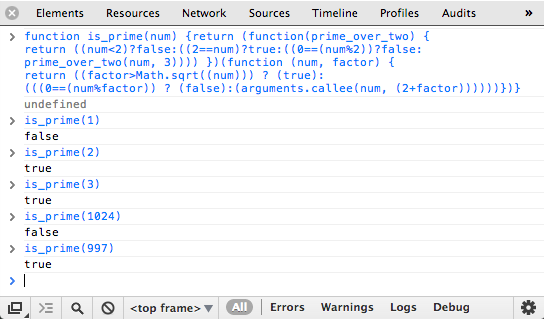
\includegraphics[scale=0.65]{Graphics/primality_test.png}
\caption{Compiled Lispish program for naive primality checking, being tested in Google Chrome JavaScript console and yielding right results.}
\label{fig:primality-javascript-test}
\end{figure}


Figure ~\ref{fig:primality-javascript-test} illustrates testing of the naive primality test program as it is fed into the Google Chrome's JavaScript console. 
At the moment of pasting the translator's output to the console, the console yields \texttt{undefined}, meaning that a function has been succesfully parsed and defined as \texttt{is\_prime(num)}. 

The \texttt{{is\_prime}} function is then tested for the first three natural numbers: $1, \ 2, \ 3 $. 1 evaluate to false, whereas the first two prime numbers, 2 and 3 evaluate to true. We then test the prime 997, which also correctly evaluates to true and 1024 which correctly evaluates to false. 
As this paper does not intend to prove the correctnes of the results of the JavaScript programs that the users of the translator writes, we can therefore conclude this test by saying that the translator produced correct JavaScript code. 

\subsection{Deploying and Using Lispish}
The end goal of this project was to be able to compile a source Lispish program to an equivalent JavaScript program.
It is, however, not ideal to have to perform compilation in an interactive REPL, where Clojure environment is set up. 

To solve this problem, the Lispish compiler is compiled as a standalone JAR file that can be executed in any environment equipped with the Java Runtime Environment. This is possible as the JAR file bundles the Clojure language itself, as well as all of its dependencies and our Lispish compiler. It exposes the application through a simple static main method, which serves as an entry point to programs execution, similarly to standard Java applications. 

There are three simple ways to compile a Lispish program to JavaScript. 

The first method is to execute the Lispish jar file and provide simple source code as a command line argument.

\subsubsection{Code as argument}

\begin{verbatim}
bash$ java -jar lispish-1.0.jar "(+ 2 2)"
Emit Lispish:  (+ 2 2)
Emit-list head:  + , tail:  (2 2)
Emit-op, head:  + , tail:  (2 2)
Emit Lispish:  2
Emit Lispish:  2
(2+2)
\end{verbatim}

Given as an input a prefix s-expression of (+ 2 2), the program yields an expected result, which is an equivalent in-fix (2+2).

This approach is fine for trivial examples that do not span across multiple lines, it is however not optimal when we want to compile a Lispish program file to an equivalent JS. 
It, therefore, only supports compiling programs made of a single s-expression like in the example above, meaning it will not compile two \texttt{defn} forms or two separate s-expressions that are not part of the same list. 

\subsubsection{Source (Lispish) and destination (JavaScript) file as argument}

In order to compile a Lispish source file to an equivalent JavaScript source file, our compiler accepts two command line options:

\begin{verbatim}
["-in" "--input" "REQUIRED: Path to Lispish source code."]
["-out" "--output" "OPTIONAL: Path to JavaScript output file."]
\end{verbatim}

\texttt{-in} or equivalently \texttt{--input}, that should follow with a path to a Lispish source file, as well as an optional 
\texttt{-out} or equivalently \texttt{--output}, that should follow with the name of the output source file. 

To demonstrate how compilation of one source file to another is performed, figure ~\ref{fig:primality-checking-input} illustrates the content of the \texttt{test.lispish} file containing the same example of naive primality checking program written in Lispish, used in the implementation section. 

We can then execute the compiler passing in the \texttt{--input} and \texttt{--output} arguments, as follows.

$$  \texttt{bash\$ java -jar lispish-1.0.jar --input test.lispish --out test.js} $$

The \texttt{--input} argument specifies path to the \texttt{test.lispish} file and \texttt{--output} argument is the path of the file to be generated.
The compiler will print out all of the computation steps to the console, but the final result, that is, the JavaScript output, will be written to the file specified in the \texttt{--output} path.

Figure ~\ref{fig:primality-checking-output} illustrates the content of the generated \texttt{test.js} file with the JavaScript equivalent of the previously shown Lispish, naive primality testing, program. 

I have purposely ommited the recursive trace of the compilation, as the recursion is invoked multiple times and it produces a very long output. 
The recursive trace is attached to the appendix ~\ref{primality-trace-appendix}. It gives a very good idea how a more complex program gets translated by outputting each one of the forms as a string, also providing name of the function responsible for translating it. 

As we can see, the Google Chrome web browsers console can evaluate the function and when executed with parameters, it yields the right result. 

\subsection{Automating tests with clojure.test API}
In order to ensure that the compiler is naturally expanded and all of the of regression tests are performed whenever a new language construct is added, I have decided to use the Test Driven Development methodology to approach this project. 
The tool to support me in the task of TDD I used was the clojure.test API.
clojure.test API\cite{clojure.test:2011:Site} is a unit testing framework that provides a set of in-built forms, particularly the \texttt{(is )} macro that allows to perform boolean assertions on arbitrary expressions. 

\begin{quote}
\begin{verbatim}
(deftest factorial-example
  (is (= 
         "function factorial(n) {return 
          ((n<2) ? (1):((n*factorial(((n-1))))))}"
         (lisp-to-js 
           "(defn factorial [n] 
              (if (< n 2) 1 (* n (factorial (- n 1)))))"))))
\end{verbatim}
\end{quote}

The above snippet is just one out of many tests included in appendix ~\ref{tests-appendix}. 

\subsection{Writing Lispish programs that interact with JavaScript functions}
As a consequence of Lispish design, the language allows for forms that begin with an arbitrary string as a function name. During the translation, the expression with an arbitrary string as a function name is translated to a JavaScript function call with the same name. This allows the user of the language to use JavaScript built-in function names in their Lispish source code. An example of this has been illustrated in the example show on figure ~\ref{fig:primality-checking-input}, where at some point of the computation, the Math.sqrt has been invoked. 

\begin{figure}[ht]
\begin{verbatim}
(defn emit-call [head [name args & rest]]
  (println "Emit-call, name: " name ", args: " args ", rest: " rest)
  (str name "("
       (if (nil? rest)
         (str "(" (emit args) ")")
         (str (str (emit args)) ", " 
         	(clojure.string/join ", " (map emit rest)))) ")"))
\end{verbatim}
\caption{emit-call source code}
\label{fig:emit-call-code}
\end{figure}


Figure ~\ref{fig:emit-cond-code} illustrates the \texttt{emit-call} function that is responsible for generating JavaScript code for recursive calls, as well as functions with arbitrary names, used for interacting with the browser and in-built JavaScript functions. 
As with the function responsible for generating code for JavaScript functions, it concatenates the optional function name, used here for invoking in-built JavaScript functions, with the emitted arguments to that function.
In case if a Lispish form begins with a recursive call, the JavaScript \texttt{arguments.callee} is passed as a function name to the above \texttt{emit-call}.
When generated, it outputs JS of the form of \texttt{arguments.callee(x, y, z)}, which tells the JS interpreter to recursively invoke the function with arguments \texttt{x, y, z}.

At first the emit-call might seem like a flaw, but it's a powerful feature, as it allows for invoking JavaScript functions responsible for interacting with the browser. 

\section{Writing Lispish programs using jQuery functions to interact with the browser's Document Object Model (DOM)}
The in-built JavaScript functions that provide an interface for manipulating content of the Document Object Model are inherently imperative.
For example, modifying a content of a \texttt{<div id=\"content\">test</div>} element requires us to use an assignment operator that will modify the state of the DOM. 

$$ \texttt{document.getElementById("test").innerHTML = "some text";} $$


The JavaScript that is generated out of Lispish does not allow for imperative assignments, as an assignment is done by means of an an argument passed to an anonymous function, which binds to the functions argument, as in the following 
example:  

\begin{verbatim}
(function(element) { element.innerHTML("some text") })(".test")
\end{verbatim}


This code would fail in JavaScript, as the \texttt{.innerHTML} is an object's property. Lispish being a non object-oriented, functional language, does not provide this functionality and therefore for it to work, \texttt{innerHTML} would have to be a function.

As a coincidence, there exist JavaScript libraries, that are in fact very popular and provide wrappers over the standard JavaScript functions.
An example of such library is a very popular jQuery\cite{jquery}. 
One of the many functionalities that jQuery provides, is the possibility to modify content of a DOM element by passing the new content to a function.
Similarly to the standard JS \texttt{.innerHTML} property, we can use jQuery's \texttt{.html()} function, that takes the new content as an argument and performs the DOM update internally. 

\begin{verbatim}
(function(x) { return x.html(("test")) })($((".someDiv")))
\end{verbatim}

The above code snippet has been generated from the following Lispish code:

\begin{verbatim}
(let [x ($(".participation"))] (x.html "test"))
\end{verbatim}

The JavaScript functions takes a jQuery \texttt{\$(".someDiv")} DOM node object and passes it as an argument to the preceding anonymous function.
It then invokes the \texttt{.html()} function with the text \texttt{test} as an argument, which replaces the content of the DIV with the text.









